\documentclass[11pt]{article}
\usepackage[margin=2.3cm]{geometry}
\usepackage{amsmath,amssymb,amsthm,booktabs,graphicx,longtable,url,hyperref,caption,float}
\newtheorem{definition}{Definition}
\title{Supplementary material for\\ \emph{From benchmark to pathway: a dynamic fuzzy soft set framework for circularity readiness and end-of-life photovoltaic strategy selection in the European Union}}
\author{Muhammad Haris Saeed\\ Department of Chemistry, University of Management and Technology, Lahore 54700, Pakistan}
\date{}
\begin{document}\maketitle

\section*{S1. Dynamic fuzzy soft sets: operators used in the main text}
Notation follows Saeed (2025) and Saeed et al.\ (2026). Let $\mathcal{S}_f$ and $\mathcal{G}_f$ be DFSSs over $(U,E,T)$ with active sets $A_t,B_t$ and memberships $\mu_{t,e},\nu_{t,e}$.

\begin{definition}[Dynamic fuzzy soft subset] $\mathcal{S}_f\subseteq\mathcal{G}_f$ iff for all $t\in T$: $A_t\subseteq B_t$ and $\mu_{t,e}(u)\le\nu_{t,e}(u)$ for all $e\in A_t$, $u\in U$.\end{definition}
\begin{definition}[Union, intersection, complement] $(\mathcal{S}_f\cup\mathcal{G}_f)(t)=(A_t\cup B_t,\ \max(\mu_{t,e},\nu_{t,e}))$ with missing memberships taken as $0$; $(\mathcal{S}_f\cap\mathcal{G}_f)(t)=(A_t\cap B_t,\ \min(\mu_{t,e},\nu_{t,e}))$; $(\mathcal{S}_f)^c(t)=(A_t,\ 1-\mu_{t,e})$.\end{definition}
\begin{definition}[Time-slice and parametric reduction] For $T'\subseteq T$, $\mathcal{S}_f|_{T'}=\{(t,A_t,F_t):t\in T'\}$; for relevance sets $R_t\subseteq A_t$, $\mathcal{S}_f^{R}=\{(t,R_t,F_t|_{R_t})\}$. Both commute with union and intersection.\end{definition}

\paragraph{Reduction properties used in the paper.} (i) If $A_t=A$ for all $t$, Eq.~(2) of the main text reduces to a time-fuzzy soft set evaluation and, with equal weights and unit confidence, the Phase-3 score equals the pooled composite B1. (ii) Hence the divergence between DFSS and B1 vanishes when $|A_t|$ is constant and weights and confidence are uniform; with dimension-balanced weights and flag-based confidence the agreement is close but not exact, which is what Scenario S1 (near-constant cardinality; $\tau_b=0.97$ against B1) shows empirically. (iii) The decomposition of Eq.~(3) is exact by construction; its two terms are the parametric reduction of period $t_1$ to $A_{t_0}$ and the residual.

\paragraph{Confidence-weighted local aggregation.} Writing $\tilde\mu_{t,e}(u)=c_{t,e}(u)\mu_{t,e}(u)$ and $\tilde w_{t,e}(u)=w_{t,e}c_{t,e}(u)$, Eq.~(2) is the ordinary weighted mean with observation-specific weights; it is monotone in $\mu$, bounded in $[0,1]$, and reduces to the DFSS Phase-2 mean when $c\equiv1$.

\paragraph{Fuzzy arithmetic in Layer C.} For triangular fuzzy numbers $\tilde a=(l,m,r)$: addition and positive scalar multiplication are componentwise; benefit normalisation divides by the maximum upper bound $u^\ast$; cost normalisation uses $(l^\ast/u,\,l^\ast/m,\,l^\ast/l)$ after shifting all values to be strictly positive; the graded mean integration representation is $(l+4m+u)/6$.

\section*{S1.1 Supplementary figures}
\begin{figure}[H]\centering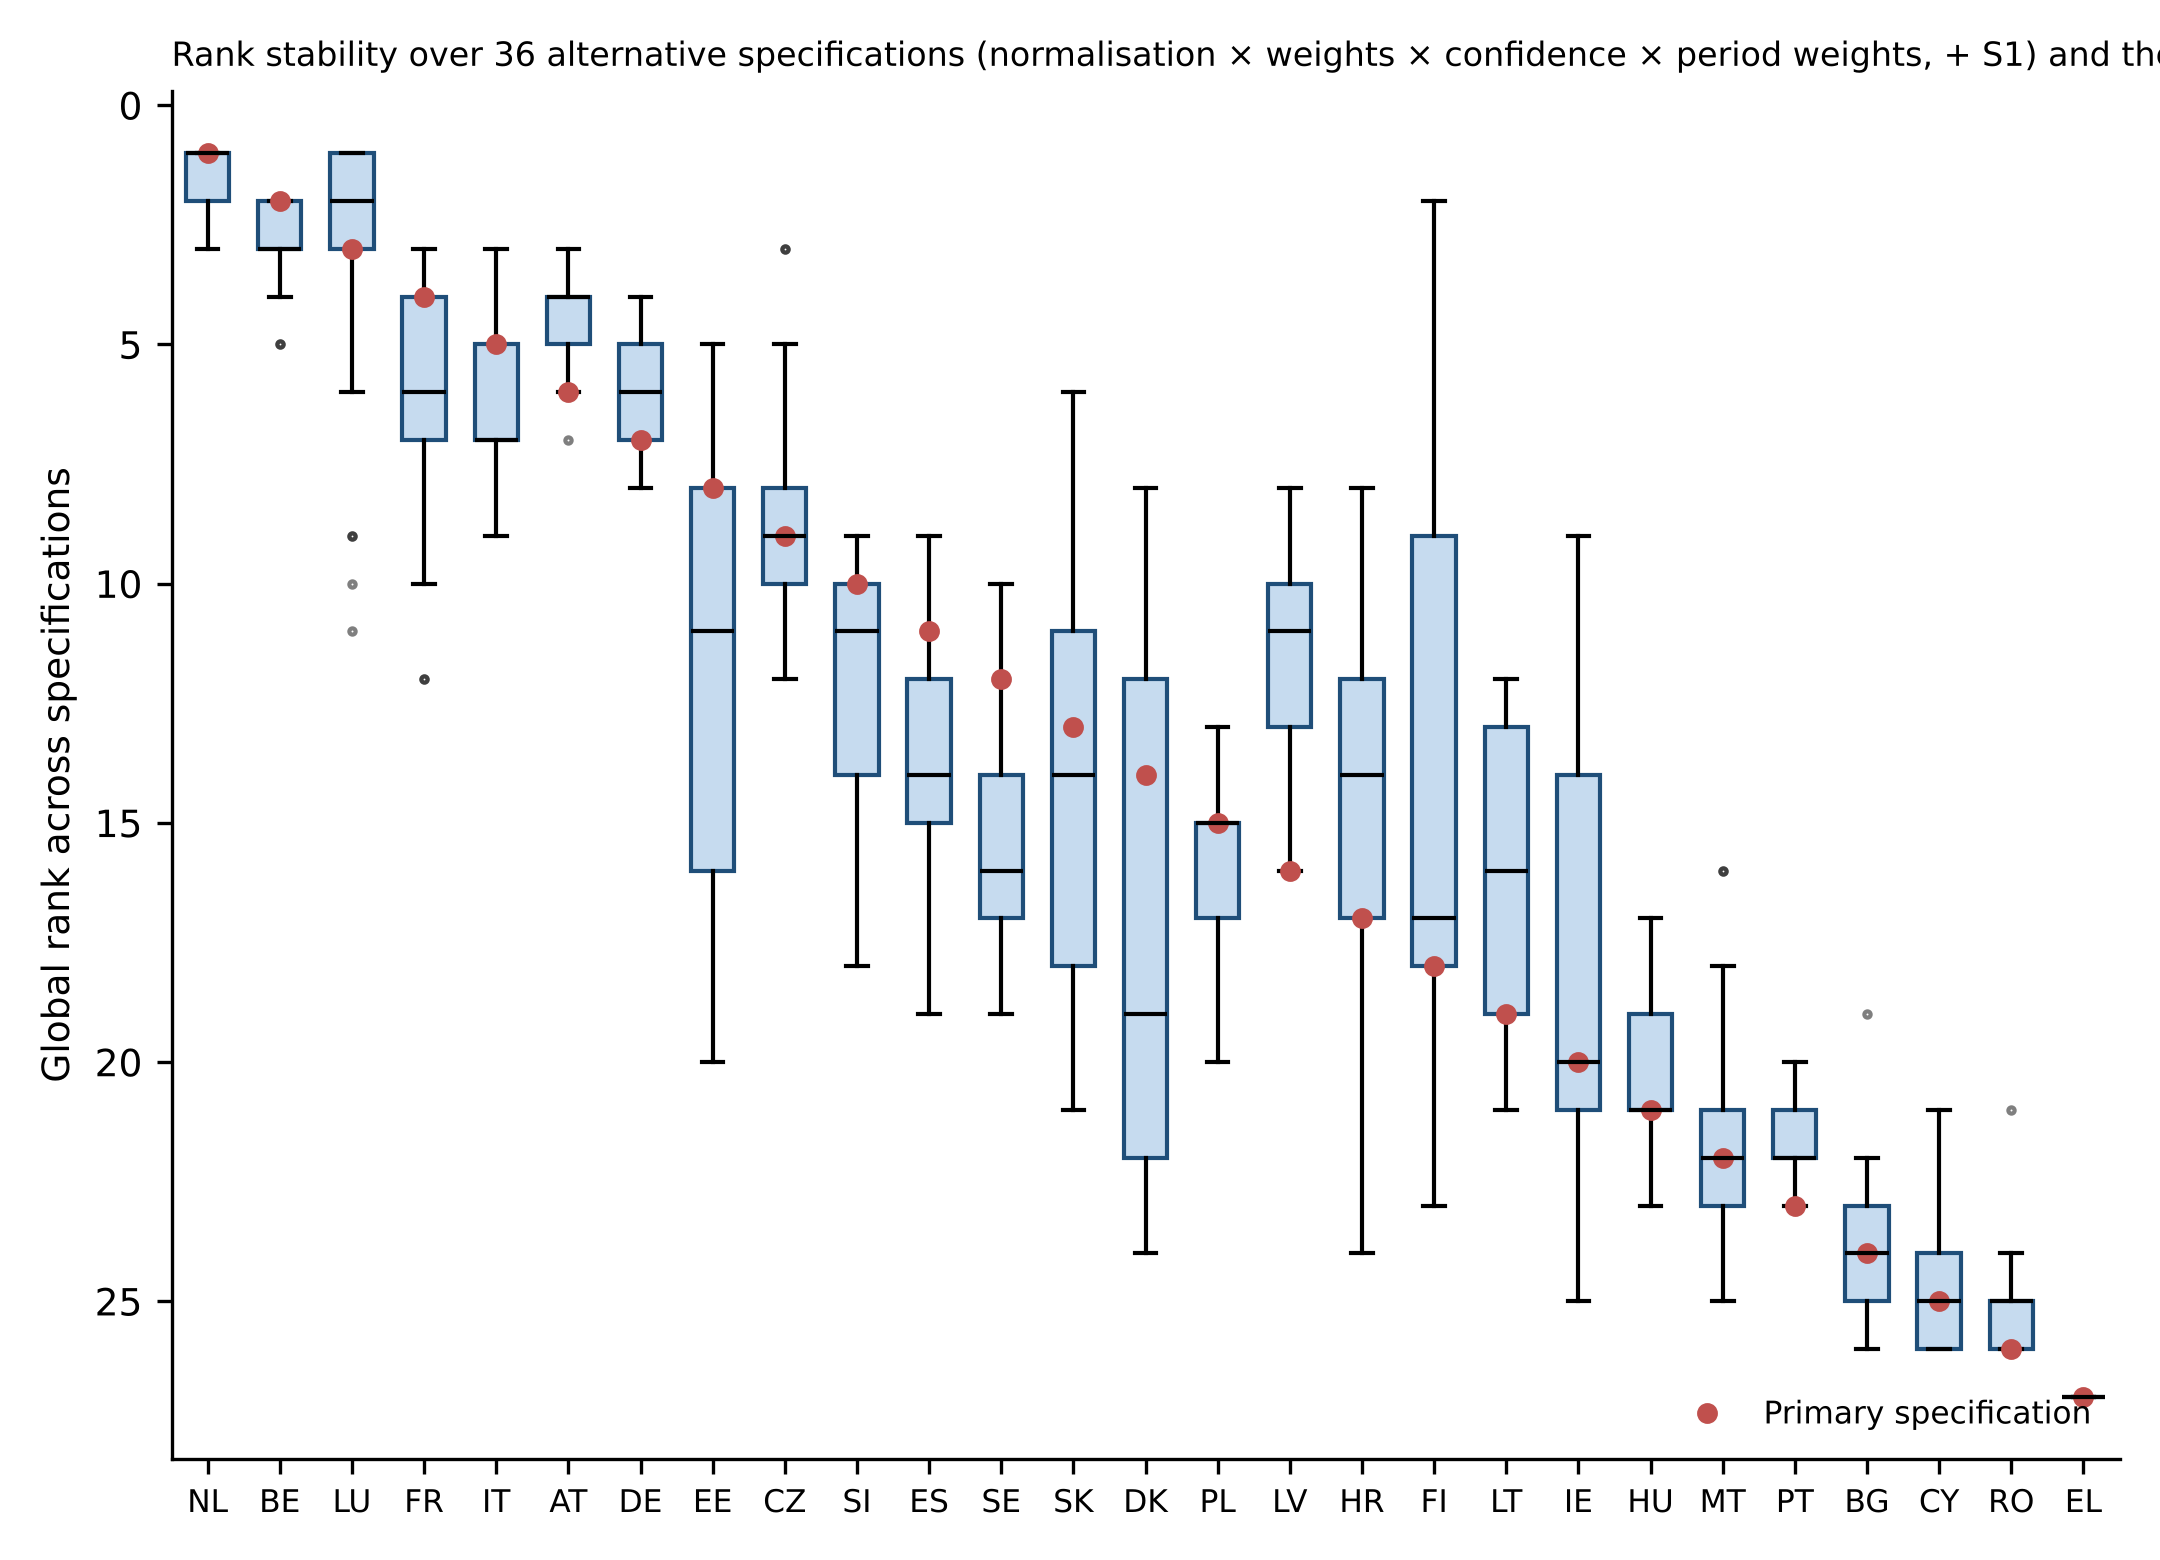
\includegraphics[width=0.95\textwidth]{figs/fig6_sensitivity_S2.png}
\caption*{Figure S1. Global rank of each member state across the 36 alternative specifications of the sensitivity grid and Scenario S1 (boxes) and under the primary specification (red).}\end{figure}
\begin{figure}[H]\centering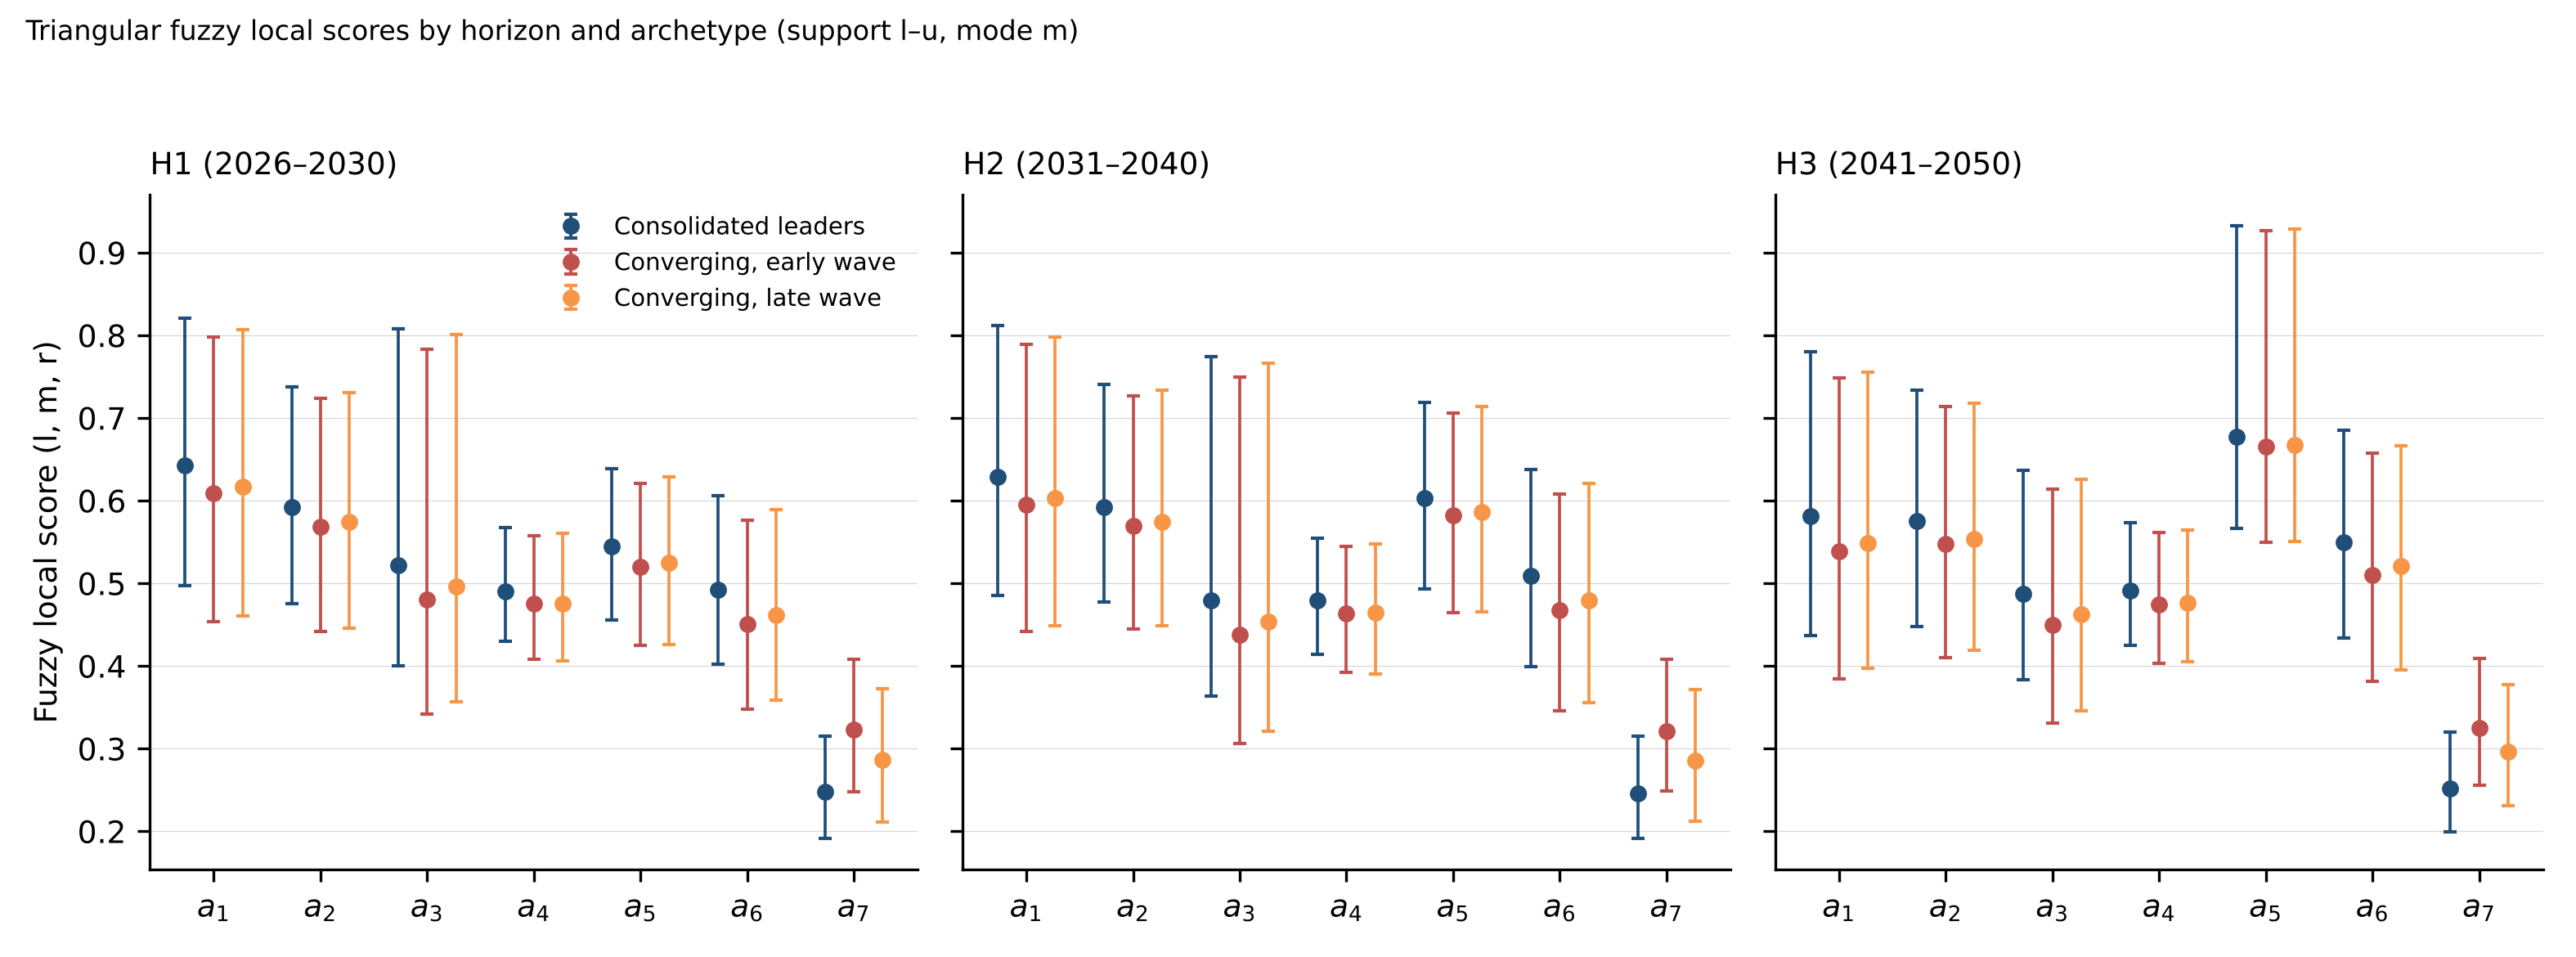
\includegraphics[width=0.95\textwidth]{figs/fig13_fuzzy_scores.png}
\caption*{Figure S2. Triangular fuzzy local scores of the seven strategies $a_1$--$a_7$ by horizon and archetype (L, EW, LW; support $l$--$r$, mode $m$).}\end{figure}

\section*{S2. Data, parameters and code}
\subsection*{S2.1 Eurostat datasets}
Circular economy indicators: cei\_pc020, cei\_pc030, cei\_pc031, cei\_pc032, cei\_pc034, cei\_pc035, cei\_pc040, cei\_pc050, cei\_wm010, cei\_wm011, cei\_wm020 (W1501), cei\_wm060, cei\_srm030, cei\_cie011 (PC\_EMP\_FTE), cei\_cie012 (INV, GVA; PC\_GDP), cei\_cie020 (P\_MHAB), cei\_gsr010 (SWS, P\_HAB), cei\_gsr011, cei\_gsr030. PV capacity: nrg\_inf\_epcrw (RA420, CAP\_NET\_ELC, MW). WEEE: env\_waselee (EE\_CPV\_PVP, COL, T; ten-category scope of Annex I, reference years 2016--2018) and env\_waseleeos (EE\_LE\_PVP, COL, T; six-category open scope of Annex III, 2019--2024); put-on-market tonnage from the same datasets (MKT). Population: tps00001. All retrieved through the dissemination API (JSON-stat 2.0) on 20 October 2026, including observation status flags.

\subsection*{S2.2 Active parameter sets}
Scenario S2: $A_{2012}=A_{2016}=\{$WGDP, MW, RRMW, RRAW, RRPW, RRWEEE, CMU, INV, GVA, EMP, PAT$\}$; $A_{2020}=\{$WGDP, MW, RRMW, RRPW, RRWEEE, CMU, INV, GVA, EMP, PAT, FW$\}$; $A_{2023}=\{$MF, RP, WG, WGDP, MW, FW, PW, PPW, RRMW, RRPW, RRWEEE, CMU, INV, GVA, EMP, CF, GHG, MID$\}$. Scenario S1: all indicators reported by $\ge22$ member states in the window.

\subsection*{S2.3 Layer B parameters}
Weibull $F(t)=1-\exp[-(t/\eta)^{\alpha}]$ with characteristic life $\eta=30$ yr (IRENA/IEA-PVPS 2016 convention); shapes: early-loss 2.4928, regular-loss 5.3759. Calibrated early share $\pi=0.18$ (pooled log-least-squares on 71 country-years with $>100$ t collected, 2016--2024, Annex-I category EE\_CPV\_PVP for 2016--2018 and open-scope Annex-III category EE\_LE\_PVP for 2019--2024; 128 country-years with positive collection; HU-2018 excluded). Country-specific fits (three or more qualifying years): DE 0.05, CZ 0.03, BE 0.10, ES 0.00, IT 0.11, NL 0.14, PT 0.16, FR 0.28, PL 0.89. Mass check: Eurostat PV modules put on the market (t) versus capacity additions times vintage mass factor, 107 country-years, median ratio 0.97, IQR 0.72--1.30. Mass per MW by vintage: 140 (1990), 120 (2000), 100 (2010), 85 (2016), 65 (2020), 55 (2024), 42 (2050) t/MW, linearly interpolated (IRENA/IEA-PVPS 2016 exponential fit; current module data sheets). Composition (mass shares, IRENA/IEA-PVPS 2016): glass 0.755, polymers 0.10, aluminium 0.08, silicon 0.05, copper 0.010, silver 0.0005, other 0.0045. Interior capacity reporting gaps (DK 2014--2017, 2019; LU 2018--2020; LV 2017; RO 2023) linearly interpolated. Monte Carlo: 600 draws.

\subsection*{S2.4 Layer C literature-derived criterion values}
Triangular fuzzy numbers $(l,m,r)$ per alternative and horizon for $C_5$ net cost (EUR/t), $C_6$ quality-weighted recovery (\%), $C_7$ avoided GHG (kg CO$_2$e/t), $C_8$ CRM recovery (\%), $C_9$ employment (FTE/kt) are listed in the accompanying workbook \texttt{LayerC\_results.xlsx}, sheet D6, and in \texttt{code/layer\_c.py}. Anchors: D'Adamo et al. (2017) recycling cost 8--19 EUR/m$^2$; Markert et al. (2020) FRELP private end-of-life cost USD 6.7/m$^2$ and recovered-material value USD 13.6/m$^2$, with FRELP yields Al 96\,\%, glass 98\,\%, Cu 75\,\%, Si 39\,\%, Ag 11\,\% (Latunussa et al. 2016); Cucchiella et al. (2015); Deng et al. (2019); Heath et al. (2020); Tsanakas et al. (2020); Maani et al. (2020). Avoided-GHG values are relative ranges anchored on these LCAs and are subject to the $\pm20\,\%$ perturbation analysis.

\subsection*{S2.5 Code}
\texttt{eurostat.py} (API client), \texttt{build\_panel.py} (panel and active sets), \texttt{layer\_a.py}, \texttt{layer\_b.py}, \texttt{layer\_c.py} (models), \texttt{figures\_a/b/c.py} and \texttt{make\_tables.py} (outputs). Full pipeline: \texttt{python3 build\_panel.py \&\& python3 layer\_a.py \&\& python3 layer\_b.py \&\& python3 layer\_c.py}. Python 3.12, pandas 3.0, scikit-learn 1.8, scipy 1.17.

\subsection*{S2.6 Institutional proxies}
Scripts \texttt{layer\_c\_proxies.py} builds the country capacity indices (\texttt{results/C\_country\_capacity.csv}), archetype capacities and the fuzzy feasibilities (\texttt{results/C\_institutional\_proxy.csv}) from Eurostat env\_waseleeos (EE6 and EE\_LE\_PVP), the CE monitoring framework panel and the World Bank WGI API (GOV\_WGI\_RQ.EST, GOV\_WGI\_RL.EST, 2021--2023 means). Raw and normalised indicator values for all 27 member states are in \texttt{results/C\_proxies\_raw.csv} and \texttt{C\_proxies\_norm.csv}.

\section*{S3. Requirement matrix and Delphi protocol}
\subsection*{S3.1 Requirement matrix $\rho(a,c)$: rationale by alternative}
\begin{description}
\item[$a_1$ Repair and refurbishment] needs preparing-for-reuse standards and re-certification rules (C1 = 0.75), refurbishers and a used-module market (C3 = 0.75), and buyer acceptance of used modules (C4 = 0.75, rising to 1.00 in H3 when the vintages reaching end of life are old) (Tsanakas et al.\ 2020). Enforcement matters less (C2 = 0.50).
\item[$a_2$ Cascaded second use] is enabled by repowering rules and warranty transfer (C1 = 0.75) and by second-use demand (C3 = 0.50; C4 = 0.50 rising to 0.75 in H3).
\item[$a_3$ Export for second life] hinges on the used-equipment/waste boundary and shipment rules (C1 = 1.00) and on their enforcement (C2 = 1.00); it needs only traders (C3 = 0.25) and modest acceptance (C4 = 0.50).
\item[$a_4$ Bulk mechanical recycling] is already mandated by the WEEE Directive (C1 = 0.50, C2 = 0.50) and needs treatment capacity (C3 = 0.75); public acceptance is not binding (C4 = 0.25).
\item[$a_5$ High-value recycling] needs recovery targets or CRM crediting (C1 = 0.75) and, above all, recyclers and secondary-material buyers (C3 = 1.00 in H1, 0.75 in H2, 0.50 in H3 as the technology matures; Heath et al.\ 2020; Deng et al.\ 2019).
\item[$a_6$ Formalised take-back] needs extended-producer-responsibility (EPR) scheme design (C1 = 0.75), certified collection and leakage control (C2 = 0.75), installer and producer-responsibility-organisation (PRO) actors (C3 = 0.75, falling to 0.50 in H3 once networks exist) and willingness of owners to hand over modules (C4 = 0.75).
\item[$a_7$ Landfill/incineration] is the default where regulation, enforcement and participation are weak; strong institutions reduce its feasibility (inverse entries C1 = C2 = 1.00, C4 = 0.75); it needs little actor capacity (C3 = 0.25).
\end{description}

\subsection*{S3.2 Delphi protocol for expert validation}
A two-round Delphi instrument was designed to elicit C1--C4 for every alternative, criterion and horizon on a five-level linguistic scale (VL, L, M, H, VH, mapped to the triangular fuzzy numbers $(0,0,0.25)$, $(0,0.25,0.5)$, $(0.25,0.5,0.75)$, $(0.5,0.75,1)$ and $(0.75,1,1)$ in \texttt{code/layer\_c.py}) from a panel of regulators, producer-responsibility organisations, installers, recyclers and researchers with experience in EU member states; Round 1 (20--30 minutes) also elicits criterion importance (1--9) and overall feasibility by member-state group; Round 2 presents the panel's aggregated ratings for revision. The instrument is provided as \texttt{Delphi\_Round1\_PV\_EoL\_questionnaire.docx} and as a Google Forms builder script; responses are ingested from \texttt{data/expert\_ratings.csv} (columns: expert\_id, horizon, archetype, alternative, criterion, rating) by \texttt{ingest\_forms.py}, after which \texttt{layer\_c.py} reports the Kendall agreement between proxy-based and expert-based rankings, a fuzzy consensus index and leave-one-expert-out stability. Recruitment for this study did not reach an adequate panel size before submission; the protocol is reported so that the proxy-based feasibilities can be tested.
\end{document}
